\documentclass[titlepage,a4paper,oneside]{article}
\usepackage[utf8]{inputenc}
\usepackage{amsmath}
\usepackage{mathabx}
\usepackage{graphicx}
\usepackage{minted}
\usepackage{booktabs}
\usepackage[english,spanish,es-noindentfirst,es-nosectiondot,es-nolists,
es-noshorthands,es-lcroman,es-tabla]{babel}
\usepackage{lmodern}             % Use Latin Modern fonts
\usepackage[T1]{fontenc}         % Better output when a diacritic/accent is used
\usepackage[utf8]{inputenc}      % Allows to input accented characters
\usepackage{textcomp}            % Avoid conflicts with siunitx and microtype
\usepackage{microtype}           % Improves justification and typography
\usepackage[svgnames]{xcolor}    % Svgnames option loads navy (blue) colour
\usepackage[hidelinks,urlcolor=blue]{hyperref}
\hypersetup{colorlinks=true, allcolors=Navy, pdfstartview={XYZ null null 1}}
\newtheorem{lemma}{Lema}
\usepackage[width=14cm,left=3.5cm,marginparwidth=3cm,marginparsep=0.35cm,
height=21cm,top=3.7cm,headsep=1cm, headheight=1.6cm,footskip=1.2cm]{geometry}
\usepackage{csquotes}
\usepackage{biblatex}
\addbibresource{informe.bib}
\usepackage[pdf]{graphviz}


\begin{document}

\begin{titlepage}
\title{
	71.14 \-- Modelos y Optimización I \-- 3er entrega\\
    \large Facultad de Ingeniería\\
	Universidad de Buenos Aires
}
\author{
	Mermet, Ignacio Javier\\
	\texttt{98153}
}
\date{Junio 2022}

\maketitle

\end{titlepage}

\tableofcontents

\newpage

\section{Análisis de las soluciones}
Si bien ambas soluciones proveen una solución con valor del objetivo $\approx 5249.622$, hay diferencias en los tiempos de ejecución, los cuales se detallan a continuación en \ref{MTZ} y \ref{Subtours}. También se detallan las diferencias en las estrategias para eliminar subtours, mediante las restricciones:

\subsection{MTZ}\label{MTZ}
Uno de los dos modelos dados por la cátedra es el ya conocido MTZ. En esta estrategia, se emplean variables enteras $U_i, i=2,\ldots,n$ que indican el orden en el cual se pasa por la ciudad $i$.

\begin{align}\label{RestriccionUs}
	u_i - u_j + \left(n-1\right) \times Y_{ij} \leq n - 2~\forall~i,j \in \text{cities} \mid i > 1,~j > 1,~j \neq i
\end{align}

La idea detrás de esta estrategia es crear un recorrido entre todas las ciudades menos la de partida, en la cual no se pueda volver para atrás. Por eso notemos que estando las ciudades indexadas desde $1$, las variables $U$ arrancan para $i=2$. Se requiere una ciudad fuera de este recorrido que cierre el tour. Esta ciudad será nuestra ciudad de partida.

La restricción \ref{RestriccionUs} no permite que se pueda ir de una ciudad con número de orden $x$ a una con número de orden $y < x$. Solo se puede volver a la ciudad inicial, por lo dicho anteriormente que no tiene esta restricción.

\begin{figure}[H]
\centering
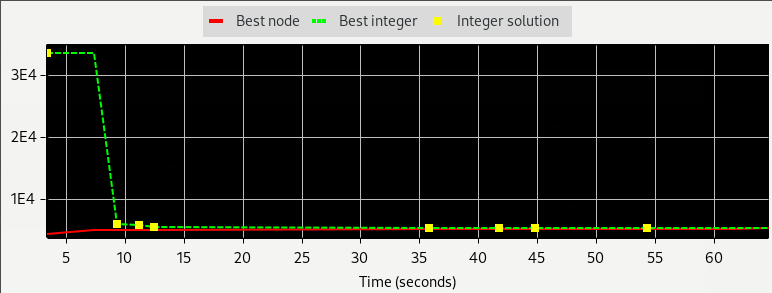
\includegraphics[width=\textwidth]{images/MTZ.png}
\caption{Gráfico de la solapa \texttt{Statistics}}
\end{figure}

\begin{figure}[H]
\begin{minted}[]{text}
Root node processing (before b&c):
  Real time             =    5.65 sec. (3495.92 ticks)
Parallel b&c, 32 threads:
  Real time             =   80.17 sec. (41031.31 ticks)
  Sync time (average)   =   23.10 sec.
  Wait time (average)   =    0.08 sec.
                          ------------
Total (root+branch&cut) =   85.82 sec. (44527.24 ticks)
\end{minted}
\caption{Fragmento de la salida bajo la solapa \texttt{Engine Log}}
\end{figure}

Notemos que la solución se alcanza en un tiempo de $85.82$ segundos (más algunos segundos de inicialización).

\subsection{Subtours}\label{Subtours}
En este segundo modelo,

Este

\begin{figure}[H]
\centering
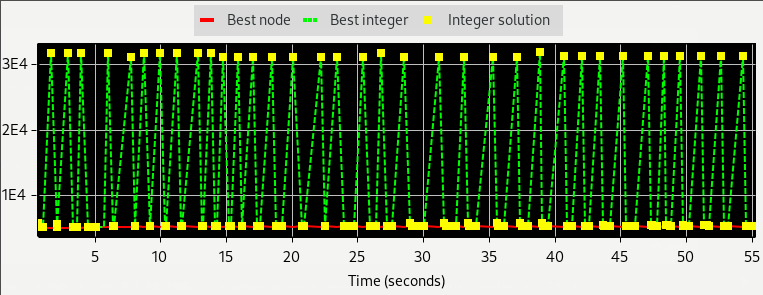
\includegraphics[width=\textwidth]{images/subtours.png}
\caption{Gráfico de la solapa \texttt{Statistics}}
\end{figure}

\begin{figure}[H]
\begin{minted}[]{text}
Root node processing (before b&c):
  Real time             =    1.46 sec. (305.17 ticks)
Parallel b&c, 32 threads:
  Real time             =    0.00 sec. (0.00 ticks)
  Sync time (average)   =    0.00 sec.
  Wait time (average)   =    0.00 sec.
                          ------------
Total (root+branch&cut) =    1.46 sec. (305.17 ticks)
\end{minted}
\caption{Fragmento de la salida bajo la solapa \texttt{Engine Log}. Notar que esto se repite más de 30 veces.}
\end{figure}

\section{Modificación de la heurística de la segunda entrega}
La heurística modificada se puede consultar en el notebook \texttt{Greedy+2opt-Problema3.ipynb}. Como resumen, utilizando una heurística de vecino más cercano, se genera un camino que empieza desde cada ciudad. Luego, se toma el de menor costo (distancia total recorrida) y se aplica 2-OPT como optimización local. En la versión de la segunda entrega se generaba una cantidad razonable de candidatos y se optimizaba localmente durante una hora como máximo. Para cumplir con las capacidades, se revisaba también que el camino fuera válido.

En esta instancia, no es necesario revisar que el camino cumpla con las restricciones de capacidad. Y dado el tamaño de la instancia del problema, se pueden generar caminos para todas las ciudades como candidatos iniciales. Esta heurística da un resultado con distancia total recorrida de $5411.213$, apenas un 3\% por encima del óptimo.

\subsection{MTZ inicializado}
\begin{figure}[H]
\centering
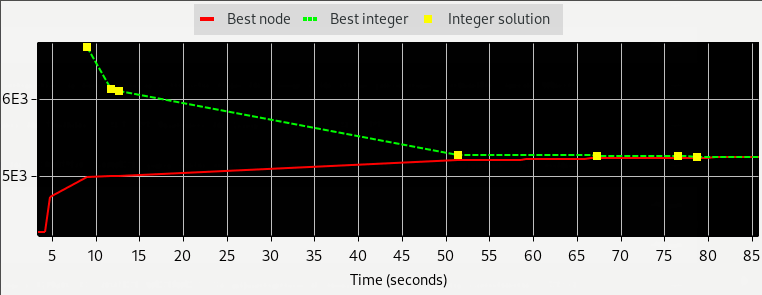
\includegraphics[width=\textwidth]{images/MTZ_init.png}
\caption{Gráfico de la solapa \texttt{Statistics}}
\end{figure}

\begin{figure}[H]
\begin{minted}[]{text}
Root node processing (before b&c):
  Real time             =    5.64 sec. (3495.92 ticks)
Parallel b&c, 32 threads:
  Real time             =   78.54 sec. (41031.31 ticks)
  Sync time (average)   =   22.18 sec.
  Wait time (average)   =    0.08 sec.
                          ------------
Total (root+branch&cut) =   84.18 sec. (44527.24 ticks)
\end{minted}
\caption{Fragmento de la salida bajo la solapa \texttt{Engine Log}}
\end{figure}

Vemos, al comparar con \ref{MTZ}, que agregar la salida de la heurística como inicialización no produce ningún cambio en la ejecución del modelo.

\subsection{Subtours inicializado}
\begin{figure}[H]
\centering
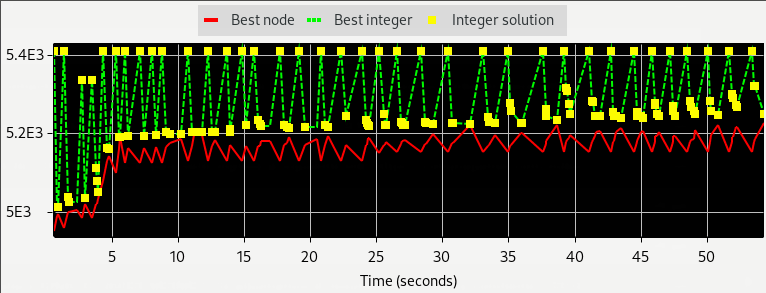
\includegraphics[width=\textwidth]{images/subtours_init.png}
\caption{Gráfico de la solapa \texttt{Statistics}}
\end{figure}

\begin{figure}[H]
\begin{minted}[]{text}
Root node processing (before b&c):
  Real time             =    1.56 sec. (276.30 ticks)
Parallel b&c, 32 threads:
  Real time             =    0.00 sec. (0.00 ticks)
  Sync time (average)   =    0.00 sec.
  Wait time (average)   =    0.00 sec.
                          ------------
Total (root+branch&cut) =    1.56 sec. (276.30 ticks)
\end{minted}
\caption{Fragmento de la salida bajo la solapa \texttt{Engine Log}. Notar que esto se repite más de 30 veces.}
\end{figure}



\printbibliography

\end{document}
